\section{Zielsetzung}
\label{sec:Zielsetzung}
Das Ziel des Versuches ist die Temperaturabhängigkeit der dynamischen 
Viskosität von destilliertem Wasser zu bestimmen. Dazu wird das 
Kugelfall\,-\,Viskosimeter nach Höppler verwendet. Außerdem wird die Reynoldszahl 
berechnet und benutzt, um herauszufinden, ob es sich um eine laminare oder
turbulente Strömung handelt.
%
%
%
\section{Theorie}
    \label{sec:Theorie}
    Bewegt sich ein Körper durch ein Medium hindurch, wirkt eine Reibungskraft 
    $\vec{F}_{R}$, die unter anderem von der Berührungsfläche und der Geschwindigkeit
    des Körpers abhängt. Je nach Strömungsart kann diese Kraft 
    unterschiedliche Abhängigkeiten haben. Bei dem Kugelfall\,-\,Viskosimeter nach 
    Höppler ist von einer laminaren Strömung auszugehen. 
    Dies wird in der Auswertung durch die
    Berechnung der Reynoldszahl überprüft. Eine experimentspeziefische 
    Reynoldszahl über ca. $2000$ weißt auf eine turbulente Strömung hin, eine die
    darunter liegt auf eine laminare Strömung (Q\cite{rz}) . Die Reynoldszahl berechnet sich
    über 
    \begin{equation}
        Re = \frac{\rho_{\text{M}} \cdot \bar{v} \cdot d}{\eta}\,. 
        \label{eqn:Reynoldszahl}
    \end{equation}
    Dabei bezeichnet $\rho_{\text{M}}$ die Dichte des Mediums, $\bar{v}$
    die mittlere Geschwindigkeit des Körpers, $d$ die charakteristische 
    Länge (beim Kugelfall\,-\,Viskosimeter ist dies der Durchmesser der Röhre)
    und $\eta$ die dynamische Viskosität des Mediums. \\
    Die Reibungskraft ist bei laminarer Strömung die Stokessche Reibung
    \begin{equation}
        \vec{F}_{R} = 6 \cdot \pi \cdot \eta \cdot v \cdot r \, , 
        \label{eqn:Stokesreibungskraft}
    \end{equation}
    hier bereits an die Symmetrie einer Kugel mit Berührungsfläche 
    $A = 6 \cdot \pi \cdot r$ angepasst, wobei $r$ der Radius der Kugel ist. 
    $\eta$ ist die dynamische Viskosität des Mediums, eine Materialkonstante und
    $v$ ist die Fallgeschwindigkeit des Körpers. \\
%
%
%
        \subsection{Kugelfall\,-\,Viskosimeter nach Höppler}
            \begin{wrapfigure}{R}{5.6cm}
                \begin{center}
                    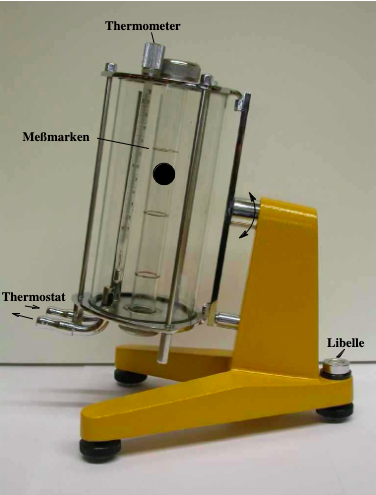
\includegraphics[width=5.5cm]{content/Viskosimeter.png}
                    %\captionstyle{indent}
                    %\setcapindent{1cm}
                    \caption[width=5.5cm]{Kugelfall\,-\,Viskosimeter\\nach Höppler. (Q\cite{anleitungV207})}
                \end{center}
                
                \label{fig:Kugelfallviskosimeter}
            \end{wrapfigure}
            Die obige beschriebene Theorie ist die Grundlage der Funktionalität des Viskosimeters 
            nach Höppler. Es besteht aus einem geschlossenen Glaszylinder, 
            welcher mit einer leichten Neigung am Fuß befestigt
            ist. Dieser Zylinder ist um 180° drehbar. Am Fuß befindet sich eine Libelle, die zur 
            richtigen Ausrichtung der Apparatur verwendet wird. 
            Innerhalb des Zylinders ist Wasser, das durch Schläuche mit einem Termostat verbunden ist,
            welches das Wasser aufheizen kann. \\
            Durch den Zylinder führt eine Glasröhre, die von außen durch Stöpsel 
            verschlossen werden kann. Auf der Glasröhre sind 3 Striche, die jeweils 
            einen Abstand von 5 \unit{\centi\meter} haben. In die innere Röhre kann
            ein Medium und eine Kugel eingefüllt werden. Durch das von außen erwärmte Wasser werden Wirbel im inneren Medium vermieden. 
            Bei diesem Experiment hat die größere verwendete Kugel näherungsweise den Durchmesser der Röhre. 
            Die leichte Neigung der Apparatur wurde gewählt, um die unkontrollierte Bewegung zu vermeiden, 
            \FloatBarrier die bei einer senkrecht herabfallenden Kugel entstehen würde. \\
            Auf die herabfallende Kugel wirken
            während des Falls drei Kräfte: Die Gravitationskraft $\vec{F}_{G} = m \cdot \vec{g}$, 
            die die Kugel nach unten beschleunigt, die Auftriebskraft $\vec{F}_{A}$ und die 
            Reibungskraft $\vec{F}_{R}$. Die Reibungskraft und Auftriebskraft wirken entgegengesetzt zur Schwerkraft. 
            Aufgrund der Kräfte beschleunigt
            die Kugel im Medium bis sie eine konstante Endgeschwindigkeit erreicht, wenn sich das Kräftegleichgewicht 
            $\vec{F}_{G} = \vec{F}_{A} + \vec{F}_{R}$ eingestellt hat.
            Die Viskosität $\eta$ wird durch die empirische Formel  
            \begin{align}
                \eta &= K \cdot \left( \rho_{K}\,-\,\rho_{M} \right) \cdot t \label{eqn:EmpirischeEtaFunktion} \\
                \Leftrightarrow K &= \frac{\eta}{ \left( \rho_{K}\,-\,\rho_{M} \right) \cdot t }
                \label{eqn:KFunktion}
            \end{align} 
            beschrieben werden. $K$ ist dabei eine Proportionalitätskonstante, $\rho_{K}$ die Dichte der Kugel und $\rho_{M}$
            die Dichte des Mediums. Die Dichte der Kugel wird durch die Formel 
            \begin{equation}
                \rho_{K} = \frac{m_{K}}{V_{K}}
                \label{eqn:DichtefunktionKugel}
            \end{equation}
            bestimmt werden, wo bei $m_{K}$ die Masse der Kugel ist und $V_{K}$ das Volumen der Kugel.
            Das Volumen wird aus dem Durchmesser $d_{K}$ durch
            \begin{equation}
                V_{K} = \frac{4}{3} \cdot \pi \cdot \left( \frac{d_{K}}{2} \right)^3
                \label{eqn:VolumenKugel}
            \end{equation} 
            berechnet werden.
            \FloatBarrier 
    %
    %
    %
    \FloatBarrier
        \subsection{Vorbereitungsaufgaben}
            \label{sec:Vorbereitungsaufgaben}
            \textbf{Wann bezeichnet man eine Strömung als "laminar"?}\\
            \\
            Eine Strömung ist dann laminar, wenn die einzelnen benachbarten Schichten 
            des Mediums ohne gegenseitige Störung aneinander vorbeigleiten und 
            keine Wirbel entstehen. \\ 
            \\
            %
            \textbf{Wie lautet die Dichte und die dynamische Viskosität von 
            destilliertem Wasser als Funktion der Temperatur?}\\
            \\
            Die Dichte von destilliertem Wasser kann unterhalb einer Temperatur von  
            $\SI{100}{\celsius}$ nicht als temperaturabhängige Formel 
            beschrieben werden.
            Die Dichte $\rho_{\text{Wasser}}$ bei der Temperatur von $\SI{20}{\celsius}$ beträgt $998.207$ 
            \unit[per-mode=fraction]{\kilo\gram\per\meter\tothe{3}}.(Q\cite{dichte})\\
            Außerdem gibt es auch keine spezielle Funktion für die dynamische
            Viskosität von destilliertem Wasser. Die Andradesche Gleichung 
            \begin{equation}
            \eta (T) = A \cdot e^{\frac{B}{T}}
            \label{eqn:AndradescheGleichung}
            \end{equation} 
            gilt auch für destilliertes Wasser. $A$ und $B$ sind Konstanten und $T$ ist die Temperatur in Kelvin. 
%\cite{sample}